\begin{figure} [htbp]
  \begin{subfigure}[b]{.49\textwidth}
   \centering
   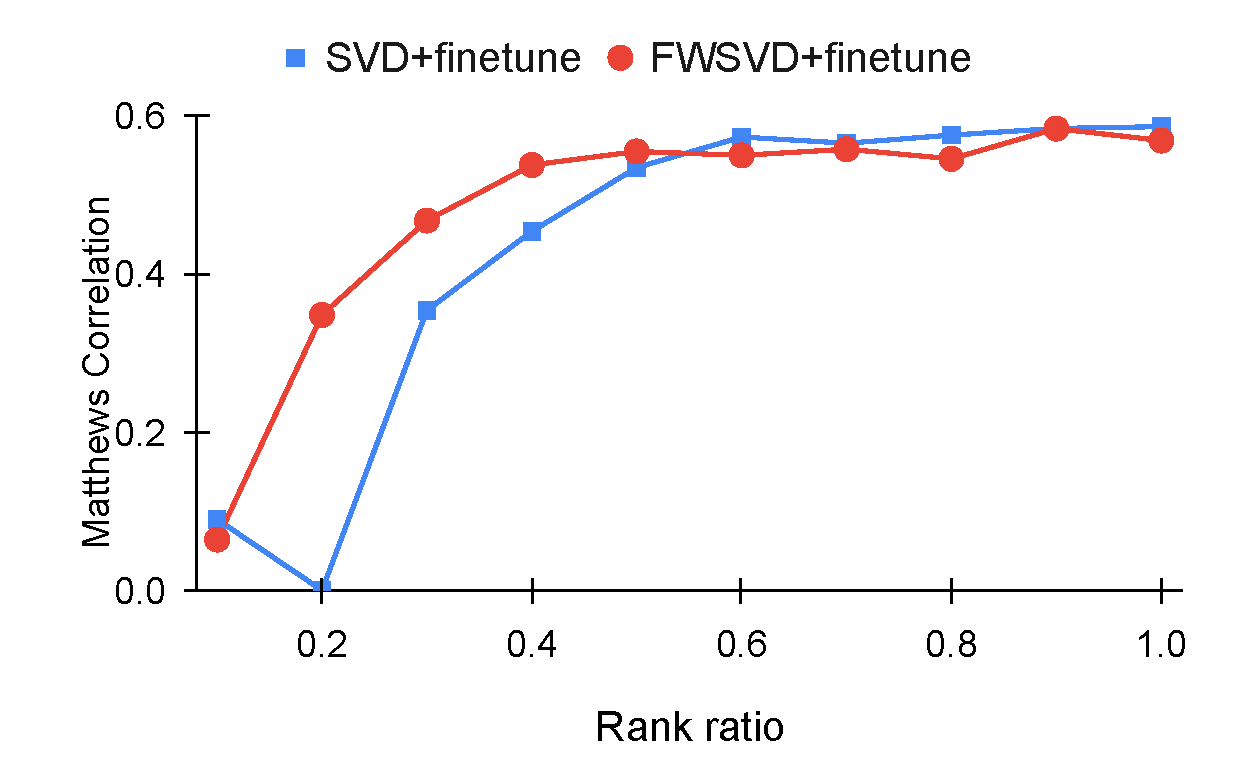
\includegraphics[width=\textwidth]{figures/app_cola_rank.pdf}
       \caption{COLA}
       \label{app:rank:cola}
       \end{subfigure}
\begin{subfigure}[b]{.49\textwidth}
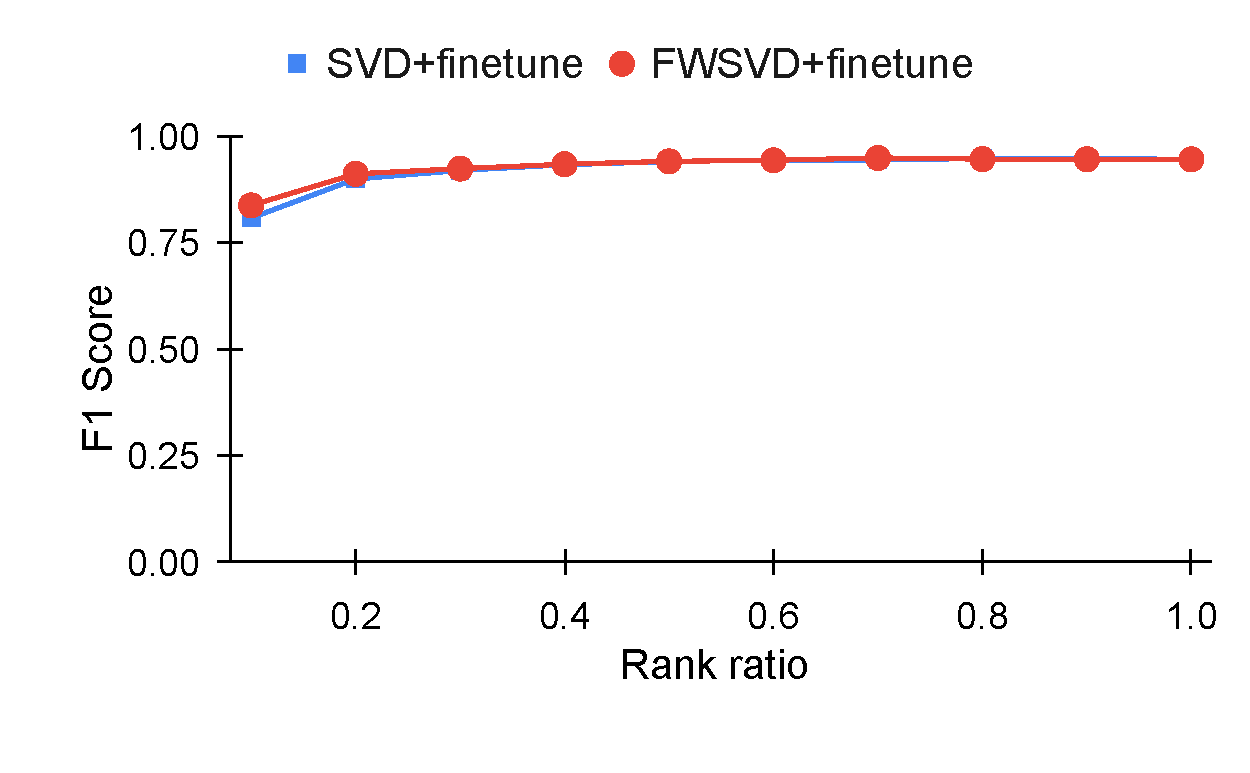
\includegraphics[width=\textwidth]{figures/app_ner_rank.pdf}
\centering
  \caption{NER (CoNLL-2003)}
   \label{app:rank:ner}
\end{subfigure}
  \begin{subfigure}[b]{.49\textwidth}
   \centering
   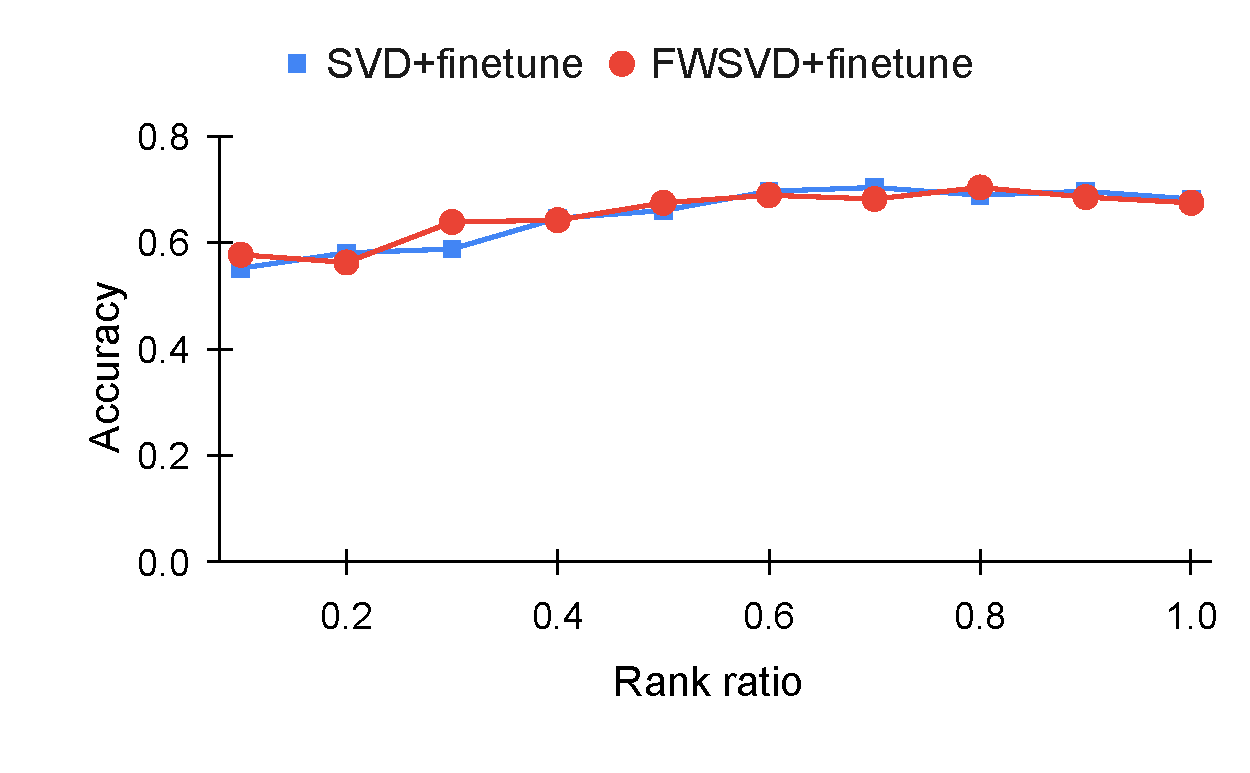
\includegraphics[width=\textwidth]{figures/app_rte_rank.pdf}
       \caption{RTE}
       \label{app:rank:0.rte}
       \end{subfigure}
\begin{subfigure}[b]{.49\textwidth}
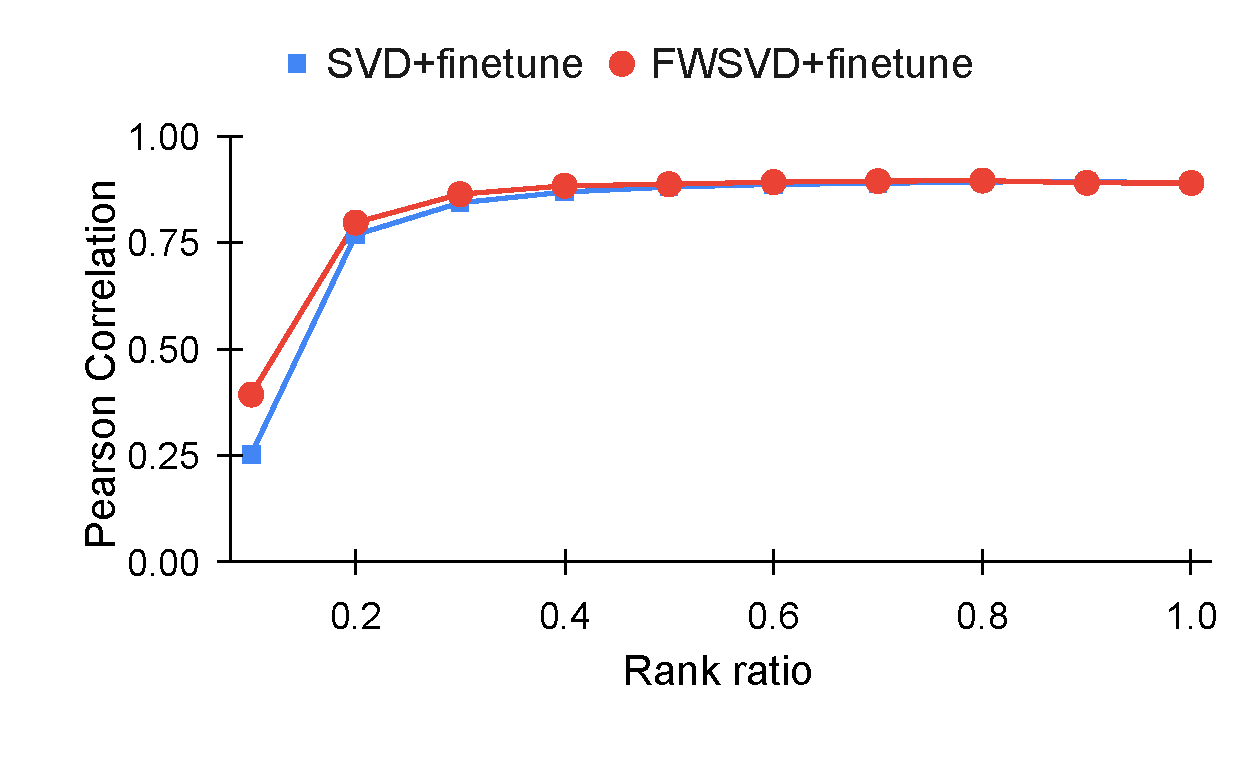
\includegraphics[width=\textwidth]{figures/app_stsb_rank.pdf}
\centering
  \caption{STS-B}
   \label{app:rank:stsb}
\end{subfigure}
\caption{FWSVD+finetune versus SVD++finetune by varying the ratio of reserved ranks. The model with a rank ratio 1.0 indicates the full-rank reconstruction with the same accuracy as the original model.
}
\label{app:rank}
\end{figure}